\section{Agent System and Evaluation Harness}
\label{sec:method}

\subsection{System Under Test: Cline Agent}
\label{sec:cline-agent}
% \subsection{被测系统：Cline 智能体}

The system under test (SUT) is Cline v3.0.51~\cite{cline2026}, an open-source coding agent that provides:
% 被测系统（SUT）为 Cline v3.0.51，一个开源编程智能体，提供：
\begin{itemize}
    \item \textbf{File tools}: \texttt{read\_file}, \texttt{write\_to\_file} for local workspace access.
    % \textbf{文件工具}：\texttt{read\_file}、\texttt{write\_to\_file}，用于本地工作区访问。
    \item \textbf{MCP bridge}: EDA tools are exposed via the \texttt{eda\_flow} MCP server (port 18891), providing \texttt{open\_session}, \texttt{run\_commands}, \texttt{run\_code}, \texttt{read\_file}, \texttt{write\_file}, \texttt{list\_files}.
    % \textbf{MCP 网桥}：EDA 工具通过 \texttt{eda\_flow} MCP 服务器（端口 18891）暴露，提供 \texttt{open\_session}、\texttt{run\_commands}、\texttt{run\_code}、\texttt{read\_file}、\texttt{write\_file}、\texttt{list\_files}。
    \item \textbf{Thinking modes}: \texttt{low}/\texttt{medium}/\texttt{high} reasoning budget (we use \texttt{low} as default).
    % \textbf{思考模式}：\texttt{low}/\texttt{medium}/\texttt{high} 三档推理预算（默认用 \texttt{low}）。
    \item \textbf{Auto-approve}: All tool calls are auto-approved (no human-in-the-loop).
    % \textbf{自动批准}：所有工具调用自动批准（无人工介入）。
\end{itemize}

\subsection{Evaluation Harness Architecture}
\label{sec:harness}
% \subsection{评测框架架构}

The evaluation harness (\texttt{run\_one.sh} / \texttt{run\_batch.sh}) implements the following pipeline (Figure~\ref{fig:pipeline}):
% 评测框架（\texttt{run\_one.sh} / \texttt{run\_batch.sh}）实现了如下流水线（图~\ref{fig:pipeline}）：

\begin{enumerate}
    \item \textbf{Deploy hook}: Copy \texttt{PreToolUse} hook to \texttt{\textasciitilde/.cline/hooks/}, configure scope to the evaluation workdir root.
    % \textbf{部署钩子}：将 \texttt{PreToolUse} 钩子拷贝到 \texttt{\textasciitilde/.cline/hooks/}，把作用范围配置为评测工作目录根。
    \item \textbf{Prepare workdir}: Create a fresh workdir, copy task assets (input files, task brief), verify no answer leakage (check.py/reference/ absent).
    % \textbf{准备工作目录}：创建全新工作目录，拷贝任务附件（输入文件、任务简述），核实无答案泄露（check.py/reference/ 不存在）。
    \item \textbf{Run agent}: Launch cline with the task prompt, model, and thinking budget. The agent reads \texttt{prompt.txt}, calls EDA tools via MCP, and writes deliverables to \texttt{outputs/}.
    % \textbf{运行智能体}：以任务提示词、模型和思考预算启动 cline。智能体读取 \texttt{prompt.txt}，通过 MCP 调用 EDA 工具，将交付件写入 \texttt{outputs/}。
    \item \textbf{Package}: After agent exit, the harness packages \texttt{outputs/} into \texttt{submit.zip} (the agent never runs zip---it only writes files).
    % \textbf{打包}：智能体退出后，框架将 \texttt{outputs/} 打包为 \texttt{submit.zip}（智能体从不执行 zip——它只写文件）。
    \item \textbf{Judge}: In a separate directory, unpack \texttt{submit.zip} and run \texttt{check.py} with the deliverable and a fresh workdir.
    % \textbf{判分}：在独立目录中解包 \texttt{submit.zip}，并以交付件和全新工作目录为参数运行 \texttt{check.py}。
    \item \textbf{Record}: Append result to \texttt{status.jsonl} (verdict, duration, hook blocks, token usage).
    % \textbf{记录}：将结果追加到 \texttt{status.jsonl}（判定、耗时、钩子拦截次数、token 用量）。
\end{enumerate}

\begin{figure}[ht]
\centering
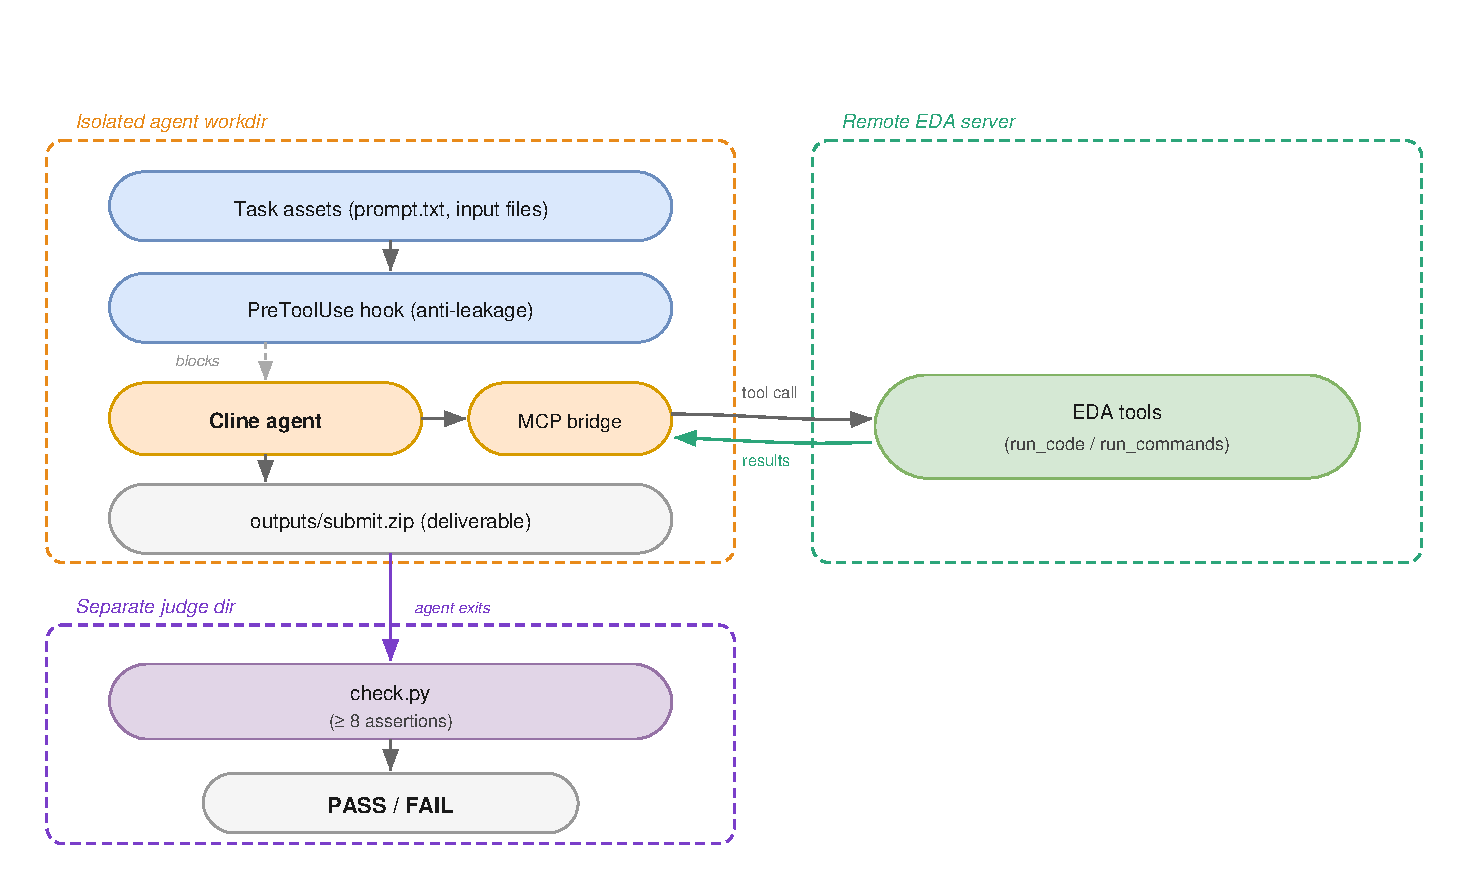
\includegraphics[width=\linewidth]{figures/pipeline.pdf}
\caption{Evaluation pipeline. The agent operates in an isolated workdir with EDA tools accessible only via MCP. The judge runs in a separate directory after agent completion.}
% \caption{评测流水线。智能体在隔离工作目录中运行，EDA 工具仅能通过 MCP 访问。判分器在智能体完成后于独立目录中运行。}
\label{fig:pipeline}
\end{figure}

\subsection{Anti-Leakage Protocol}
\label{sec:anti-leakage}
% \subsection{防泄题协议}

Answer leakage---the agent reading the answer key directly---is the single largest threat to benchmark validity. We enforce isolation through three layers:
% 答案泄露——智能体直接读取答案——是基准有效性最大的威胁。我们通过三层隔离来防范：

\begin{itemize}
    \item \textbf{Filesystem isolation}: The workdir contains only task assets and \texttt{prompt.txt}. The reference \texttt{check.py} and \texttt{reference/} directory are never copied into the workdir.
    % \textbf{文件系统隔离}：工作目录只含任务附件和 \texttt{prompt.txt}。参考 \texttt{check.py} 与 \texttt{reference/} 目录从不拷入工作目录。
    \item \textbf{PreToolUse hook}: A shell hook intercepts every tool call and blocks access to paths matching \texttt{check.py}, \texttt{\_check.py}, \texttt{reference/}, \texttt{hidden/}, and any file outside the workdir. Blocked calls return ``ACCESS RESTRICTED'' to the agent.
    % \textbf{PreToolUse 钩子}：一个 shell 钩子拦截每次工具调用，阻止访问匹配 \texttt{check.py}、\texttt{\_check.py}、\texttt{reference/}、\texttt{hidden/} 及工作目录之外的任何文件。被拦截的调用向智能体返回"ACCESS RESTRICTED"。
    \item \textbf{Scope management}: The hook scope is set to the evaluation workdir root, ensuring concurrent evaluations don't cross-access.
    % \textbf{作用域管理}：钩子作用域设为评测工作目录根，确保并发评测不会互相越权访问。
\end{itemize}

We verify isolation by counting \texttt{ACCESS RESTRICTED} events in each session log (\texttt{hook\_blocks} field in \texttt{status.jsonl}).
% 我们通过统计每份会话日志中的 \texttt{ACCESS RESTRICTED} 事件（\texttt{status.jsonl} 的 \texttt{hook\_blocks} 字段）来验证隔离是否生效。

\subsection{EDA Server Bridge}
\label{sec:eda-bridge}
% \subsection{EDA 服务器网桥}

The EDA server (10.129.32.75) provides:
% EDA 服务器（10.129.32.75）提供：
\begin{itemize}
    \item \textbf{Session management}: \texttt{open\_session} creates an isolated workdir; \texttt{close\_session} archives and removes it.
    % \textbf{会话管理}：\texttt{open\_session} 创建隔离工作目录；\texttt{close\_session} 归档并删除它。
    \item \textbf{Command execution}: \texttt{run\_commands} runs shell/EDA commands in the session workdir (bash -lc).
    % \textbf{命令执行}：\texttt{run\_commands} 在会话工作目录中运行 shell/EDA 命令（bash -lc）。
    \item \textbf{Code execution}: \texttt{run\_code} executes pyAether/SKILL/Tcl code in the appropriate EDA interpreter.
    % \textbf{代码执行}：\texttt{run\_code} 在对应的 EDA 解释器中执行 pyAether/SKILL/Tcl 代码。
    \item \textbf{File I/O}: \texttt{read\_file}/\texttt{write\_file} for EDA-side file access.
    % \textbf{文件读写}：\texttt{read\_file}/\texttt{write\_file} 用于 EDA 侧文件访问。
\end{itemize}

The agent must call \texttt{open\_session} first to obtain a workdir, then pass it to all subsequent calls. This mirrors real EDA workflow patterns where engineers open a design session before running tools.
% 智能体必须先调用 \texttt{open\_session} 取得工作目录，再将其传入所有后续调用。这映照了真实的 EDA 工作流习惯——工程师在运行工具前先打开一个设计会话。
